% Modelo de Dissertação do Mestrado em Informática da PUC - Alterado para cumprir a normalização de 2011
%\documentclass[a4paper,brazil,ruledheader,normaltoc,capchap]{abnt}

% Para impressão frente e verso (normalização 2011)
\documentclass[a4paper,brazil,ruledheader,normaltoc,capchap,twoside,openany]{abnt_pucmg_utf8}

% Não esquecer das alterações no arquivo abnt.cls
% Se estiver usando o Kile no Ubuntu o arquivo fica armazenado em /usr/share/texmf/tex/latex/abntex.
% Comentar a linha 967 
% \vspace*{30pt}% - Linha comentada para reduzir o espaçamento entre o topo da página e o título \chapter
% Alterar a linha 1143
% \vspace*{-30pt} % - Parâmetro alterado de 30pt para -30pt para reduzir o espaçamento entre o top da página e o título do apêndice
% Alterar a linha 985
%\vspace*{-30pt}\par % - Parâmetro alterado de 0pt para -30pt para reduzir o espaçamento entre o top da página e o título \chapter*
% Alterar a linha 991
% Parâmetro alterado de 45pt para 30pt para reduzir o espaçamento entre o texto e o título \chapter*

% Não esquecer das alterações no arquivo acronym.sty
% Se estiver usando o Kile no Ubuntu o arquivo fica armazenado em /usr/share/texmf-texlive/tex/latex/acronym
% Alterar a linha 225
%\item[\protect\AC@hypertarget{#1}{\acsfont{\normalfont{#2}}} --] #3% - Inserir separador entre acrônimo/descrição e remover o negrito com o normalfont

% Pacote para definir explicitamente as margens das páginas
\usepackage[a4paper,left=3cm,right=2cm,top=3cm,bottom=2cm]{geometry}

%\usepackage{units}
% Utilize da seguinte forma \unit[78,6]{mA}

% Pacote para gerenciar siglas
\usepackage[printonlyused]{acronym}

% Merge em duas células (linhas diferentes)
\usepackage{multirow}

% Pacote para citação e referências seguindo ABNT no sistema (AUTOR, Data)
%\usepackage[alf, bibjustif,abnt-emphasize=bf]{abntcite}
\usepackage[alf, abnt-emphasize=em, abnt-thesis-year=title]{abntcite}
% @article An article from a journal or magazine 
% @inproceedings An article in a conference proceedings
% Força que o tipo de ênfase no nome do simpósio seja em caixa alta
\renewcommand{\emph}{\textsc}

% Pacote para múltiplos arquivos .bib
\usepackage{multibib}
%\newcites{pub}{Refer\^encias das publica\c{c}\~oes}

% Pacote de adequação do formato ABNT para normas da PUCMinas
\usepackage{abnt-PPGInf-PUCMG}

% Pacotes utilitários
\usepackage{graphicx}

% Pacote para fixar a figura no local desejado
\usepackage{float}

% Pacote para adicionar simbolos as informações de rodapé
\usepackage[symbol]{footmisc}

\usepackage[all]{xy}
%\usepackage[tight]{subfigure}	% Permite a criação de subfiguras
\usepackage{url,amsmath}	% Permite melhorias na codificação de fórmulas
%\usepackage{amsthm}		% Permite melhorias na escrita de teoremas
\usepackage{amssymb}		% Permite utlização de simbolos matemáticos avançados

\usepackage[portuguese, linesnumbered, ruled, vlined]{algorithm2e}
\usepackage{algorithmic} 	% para algoritmos
\usepackage{listings} 		% para importação de código-fonte

% Alterar o espaçamento da margem no algoritmo
\setlength{\algomargin}{1em}

\usepackage{setspace}

% Pacote para rotação de tabelas/figuras
\usepackage{rotating}

% Pacotes para criação de cronograma/tabela colorida
\usepackage{color}
\usepackage{array}
\usepackage{longtable}
\usepackage{colortbl}
%\definecolor{lightgray}{gray}{0.9}

% Pacote para possibilitar o uso do setboolean para forçar formatos de página diferentes do padrão do documento
\usepackage{ifthen}

% Para inserir captions (nova normalização 2011)
\usepackage[size=normalsize,labelfont=bf,textfont={bf},labelsep=endash]{caption}
\captionsetup[subfloat]{labelfont=bf,textfont={bf}}

% Usado para reduzir espaçamentos entre itens (alíneas, enumerações) com o compactitem
\usepackage{paralist}

% Alterar para sequencial a numeração de figuras e tabelas
\captionsetup{figurewithin=none}
\captionsetup{tablewithin=none}

\setlength{\LTcapwidth}{\textwidth}

% Para o subsubsection aparecer no sumário 
\setcounter{tocdepth}{3}
\setcounter{secnumdepth}{3}

% Para inserir referências via links - não funciona para abntex
%\usepackage[colorlinks=true,pdfstartview=FitV,linkcolor=blue,citecolor=blue,urlcolor=blue,hyperindex,pagebackref=true,pdftex,breaklinks]{hyperref}
%\usepackage[pdftex]{hyperref}

% Para criar lista de gráficos
\floatstyle{plaintop}
\newfloat{grafico}{H}{loq}
\restylefloat*{grafico}
\floatname{grafico}{Gráfico} 

% Para gerar subfiguras usando o subfloat
\usepackage{subfig}
\newsubfloat[position=bottom,listofformat=subsimple]{grafico}

% define estilo de posicionamento na caixa
\newsavebox{\leftfig}
\newsavebox{\rightfig}

%\renewcommand{\ALG@name}{Algoritmo}
%\renewcommand{\listalgorithmname}{Lista de Algoritmos}

% Configuração de código-fonte
\lstset{extendedchars=\true, % permite acentos
 inputencoding=utf8,
 literate={\$}{{\$}}1,
 commentstyle=\it, % deixa os comentários em itálico
 stringstyle=\bf, % não lembro o que faz, mas está funcionando
 belowcaptionskip=5pt, % não lembro o que faz, mas está funcionando
 numbers=left, % coloca a numeração na esquerda
 stepnumber=1, % passos da numeração
 firstnumber=1, % primeira linha
 numberstyle=\tiny, % tamanho da fonte da numeração
 breaklines=true, % permitir quebra de linha
 frame=tb, % borda em cima e em baixo
 basicstyle=\footnotesize, % estilo básico
 stringstyle=\ttfamily, % não lembro o que faz, mas está funcionando
 showstringspaces=false, % não mostrar os espaços
 mathescape, % não lembro o que faz, mas está funcionando
 tabsize=3 % tamanho da tabulação
}
\renewcommand{\lstlistingname}{Código}
\renewcommand{\lstlistlistingname}{Lista de Códigos}
\citeoption{abnt-etal-cite=1, abnt-and-type=e}

% the bibtex style generates this command, but it's not defined
\newcommand{\optionaltextstyle}{}

%%\pdfinfo{%
%%  /Title    (TITULO DA DISSERTACAO)
%%  /Author   (Nome do aluno)
%%  /Creator  (Nome do aluno)
%%  /Producer (Kile - an Integrated LaTeX Environment - %%Version 2.0.85)
%%  /Subject  (Dissertação de Mestrado)
%% /Keywords (Palavras chave)
%%}

% PRÉ-TEXTUAIS %%
\begin{document}

% Para forçar que elementos pré-textuais (da capa até o sumário) sejam impressos no anverso da folha
\setboolean{@twoside}{false}

\autor{Lucas Simon Rodrigues Magalhães}

% Coloque o título em caixa alta. É o padrão da PUC.
% Vá no arquivo abnt-PPGInf-PUCMG.sty e procure por esse título (linha 575). Altere para o seu título em caixa alta. Isso será utilizado na folha de aprovação.
\titulo{Utilizando JavaScript no servidor para construir aplicações de alta concorrência na internet com Node.Js}

\orientador[Orientador:]{Prof. João Caram}

% Se não tiver, co-orientador, comente a próxima linha.
%\coorientador[Co-orientador:]{Professor}

% Texto
\comentario{Monografia apresentada ao Departamento de Sistemas de Informação da Pontifícia Universidade Católica de Minas Gerais,
como exigência parcial para a obtenção do título de Bacharel em Sistemas de Informação.}


% Instituição
\instituicao{Bacharelado em Sistemas de Informação \par Departamento de Sistemas de Informação \par Pontifícia Universidade Católica de Minas Gerais}

% Local
\local{Belo Horizonte}

% Data
\data{24 de Novembro de 2014}
\capa
%Para forçar que a ficha catalográfica seja impressa no verso da folha de aprovação
\setboolean{@twoside}{true}

% Gera a folha de rosto
\folhaderosto

% Ficha catalográfica
% Ficha catalográfica
% INCLUIR O ARQUIVO PDF GERADO PELA BIBLIOTECA COMO FIGURA.
\begin{figure}[h!]
	\vspace*{-3.3cm}
	\hspace*{-3cm}
%	% Suponha o nome do arquivo em pre-texto/ficha-catalografica/fichacatalografica.pdf
	\includegraphics{pre-texto/ficha-catalografica} 
	\newpage
\end{figure}

% Para forçar que elementos pré-textuais (da capa até o sumário) sejam impressos no anverso da folha
\setboolean{@twoside}{false}

% Folha de aprovação
% Termo de Aprovação

% Texto da aprovação
\textoaprovacao{Dissertacao apresentada ao Programa de Pos-Graduacao em Informatica como requisito parcial para qualificacao ao Grau de Mestre em Informatica pela Pontificia Universidade Catolica de Minas Gerais.}

% Primeira assinatura
\primeiroassina{Prof. Dr. Orientador -- PUC Minas}

% Segunda assinatura
\segundoassina{Prof.$^{a}$ Dr.$^{a}$ Membro interno -- Instituicao}

% Terceira assinatura
\terceiroassina{Prof. Dr. Membro externo -- Instituicao}

% Quarta assinatura
%\quartoassina{}

% Data da defesa
\localdia{Belo Horizonte, data da defesa.}

% Gera o termo de aprovação
\termodeaprovacao	

% Dedicatória
% Dedicatória
\newpage

% Espaçamento do topo da página até o texto da dedicatória
\vspace*{22cm}

% Espaçamento na esqueda
\hspace{8cm}\begin{minipage}{.60\textwidth}
            \textit{Dedico este trabalho à meus familiares e amigos que me acompanharam durante todo esse tempo em meus estudos, às vezes me apoiando e às vezes puxando minha orelha.}
            \end{minipage}

% Agradecimentos
% Agradecimentos
%\chapter*{Agradecimentos}
\begin{center}
	\normalsize
	\textbf{AGRADECIMENTOS}
\end{center}

  Aos meus pais, Ivam Silva Magalhães e Haydee Rodrigues Magalhães, por todo os valores, educação e estímulos aos meus estudos, profissionalmente e pessoalmente. A minha irmã Nadia Rodrigues Magalhães que nos momentos mais difíceis sempre me procurou, conversou e me apoiou de todas as formas possíveis.
  
  Ao meu amigo Igor Tadeu Camilo Rocha que me ajudou a escrever, corrigir e tornar deste um trabalho de sucesso

% Epígrafe
% Epígrafe
\newpage

% Espaçamento entre topo da página e texto da epígrafe
\vspace*{10cm}
% Espaçamento na esqueda
\hspace{4cm}\begin{minipage}{.51\textwidth}

% Texto da epígrafe
\textit{``E fazendo que se aprende a fazer aquilo que se deve aprender a fazer.'' }

%Nome do autor
\begin{flushright}\itshape Aristoteles \upshape\end{flushright}

\end{minipage}

% Resumo
% Resumo
\begin{resumo}
% Diminuir espaçamento entre título e texto
\vspace{-1cm}

% Texto do resumo: sem paragrafo, justificado, com espaçamento 1,5 cm
\onehalfspacing

\noindent
  
  
  Com o crescente número de usuários conectados a aplicações nos servidores,
  é necessário repensar no modelo de desenvolvimento de aplicações web existentes atualmente.
  Na atual arquitetura web tem-se de pensar na arquitetura do sistema, utilizar técnicas de cache e 
  investir em escalonamento de servidores.  
  
  O Node.Js propõe alterar esse paradigma com o objetivo de fornecer uma arquitetura de software 
  capaz de receber milhões de conexões simultâneas e ser facilmente escalável, 
  sem necessidade de custos exorbitantes com infraestrutura.
  
  Para validar a potencialidade do Node.Js vamos estudar o básico deste ambiente e em seguida realizar um
  estudo de caso com uma API REST, muito utilizado no serviços web. Após o estudo será desenvolvido
  dois sistemas onde iremos comparar a forma de desenvolvimento de um \textit{framework} Django e 
  do \textir{framework} Express.js para Node.Js
  
  Com os aplicativos desenvolvidos serão realizados testes de carga nos dois ambientes verificando o tempo
  de resposta e sucessos em cada requisições. E por fim vamos analisar os resultados dos testes e informar
  ao leitor a capacidade de cada sistema.

% Espaçamento para as palavras-chave
\vspace*{.75cm}

% Palavras-chave: sem parágrafo, alinhado à esquerda
\noindent Palavras-chave: Node.Js; programação orientada a eventos; Análise de desempenho.\\
% Segunda linha de palavras-chave, com espaçamento.
%\indent\hspace{2cm}Palavra.

\end{resumo}

% Abstract
% Abstract
\begin{abstract}
% Diminuir espaçamento entre título e texto
\vspace{-1cm}
% Texto do resumo, em inglês: sem paragrafo, justificado, com espaçamento 1,5 cm
\onehalfspacing
\noindent
  Texto do resumo, em ingles.

% Espaçamento para as palavras-chave
\vspace*{.75cm}

% Palavras-chave: sem parágrafo, alinhado à esquerda
\noindent Keywords: . \\
% Segunda linha de palavras-chave, com espaçamento.
%\indent\hspace{1.4cm} Keyword.

\end{abstract}

\makeatletter
\renewcommand\numberline[1]{
	\leftskip 0em
	\rightskip 1.6em
	\parfillskip -\rightskip
	\parindent 0em
	\@tempdima 2.0em
	\vspace{0em} \advance\leftskip \@tempdima \null\nobreak\hskip -\leftskip
	FIGURA \normalfont #1 -- }
\makeatother

% Lista de figuras
\listoffigures

\makeatletter
\renewcommand\numberline[1]{
	\leftskip 0em
	\rightskip 1.6em
	\parfillskip -\rightskip
	\parindent 0em
	\@tempdima 2.0em
	\vspace{0em} \advance\leftskip \@tempdima \null\nobreak\hskip -\leftskip
	TABELA \normalfont #1 -- }
\makeatother

% Lista de tabelas
\listoftables

\makeatletter
\renewcommand\numberline[1]{
	\leftskip 0em
	\rightskip 1.6em
	\parfillskip -\rightskip
	\parindent 0em
	\@tempdima 2.0em
	\vspace{0.5em} \advance\leftskip \@tempdima \null\nobreak\hskip -\leftskip
	GRÁFICO \normalfont #1 -- }
\makeatother

% Lista de graficos
\listof{grafico}{Lista de Graficos}

% Lista de siglas
% Lista de Abreviaturas e Siglas
%\chapter*{Lista de Abreviaturas e Siglas}
\chapter*{Lista de Abreviaturas e Siglas}

% Mantenha sempre em ordem alfabética.

\begin{acronym}
\acro{API} {Interface de Programação de Aplicativos, do inglês \textit{Application Programming Interface}}
\acro{CLI} {Interface para a linha de comando, do inglês \textit{Command Line Interface}}
\acro{CPU} {Unidade central de processamento, do inglês \textit{Central Processing Unit}}
\acro{CRUD} {Criar, ler, atualizar e deletar, do inglês \textit{Create, Read, Update, Destroy}}
\acro{DNS} {Sistema de nome de Domínios, do inglês \textit{Domain Name System}}
\acro{E/S} {\textit{Entrada e Saída}}
\acro{HTML} {Linguagem de marcação de hipertexto, do inglês \textit{HyperText mark-up Language}}
\acro{HTTP} {Protocolo de transferência de hipertexto, do inglês \textit{HyperText Transfer Protocol}}
\acro{JSON} {Notação de objetos Javascript, do inglês \textit{JavaScript Object Notation}}
\acro{MVR} {Modelo, visão e rotas, do inglês \textit{Model View Routes}}
\acro{MVC} {Modelo, visão e controladores, do inglês \textit{Model View Controller}}
\acro{NOSQL} {Não Somente SQL usado para definir bancos de dados não relacionais, do inglês \textit{Not Only SQL}}
\acro{NPM} {Gerenciador de pacotes do Node.js, do inglês \textit{Node Package Manager}}
\acro{PHP} {\textit{PHP: Hypertext Preprocessor}}
\acro{REST} {Transferência de Estado Representativo, do inglês \textit{Representational State Transfer}}
\acro{SSD} {Unidade de estado sólido, do inglês \textit{Solid state drives}}
\acro{SQL} {Linguagem de Consulta Estruturada, do inglês \textit{Structured Query Language}}
\acro{URI} {Identificador de recurso uniforme, do inglês \textit{Uniform Resource Identifier}}
\acro{URL} {Localizador uniformizado de recursos, do inglês \textit{Uniform Resource Locator}}
\acro{VPS} {Servidor privado virtual, do inglês \textit{Virtual Private Server}}



\acro{BER} {\textit{Bit Error Rate}}
\acro{BT} {\textit{Block Tri-diagonal}}
\acro{CG} {\textit{Conjugate Gradient}}
\acro{CSS} {\textit{Chirp Spread Spectrum}}
\acro{DCC-MAC} {\textit{Dynamic Channel Coding} MAC}
\acro{DSSS} {\textit{Direct-sequence spread spectrum}}
\acro{EP} {\textit{Embarrassingly Parallel}}
\acro{FIFO} {\textit{First In, First Out}}
\acro{FT} {\textit{Fast Fourier Transform}}
\acro{IEEE} {\textit{Institute of Electrical and Electronics Engineers}}
\acro{IR-UWB} {\textit{Impulse Radio} UWB}
\acro{IS} {\textit{Integer Sort}}
\acro{LU} {\textit{Lower-Upper Gauss-Seidel}}
\acro{MAC} {\textit{Medium Access Control}}
\acro{MB-OFDM} {\textit{Multi-Band Orthogonal Frequency Division Multiplexing}}
\acro{MG} {\textit{Multi-Grid}}
\acro{MPE} {MPI \textit{Parallel Environment}}
\acro{MPI} {Interface de passagem de mensagem, do inglês \textit{Message Passing Interface}}
\acro{NAS} {NASA \textit{Advanced Supercomputing}}
\acro{NOAH} {\textit{No Ad-Hoc Routing Agent}} 
\acro{NS-2} {\textit{Network Simulator} 2}
\acro{NoCs} {Redes-em-Chip, do inglês \textit{Networks-on-Chip}}
\acro{NPB} {NAS \textit{Parallel Benchmark}}
\acro{OpenMP} {Multi-processamento aberto, do inglês \textit{Open Multi-Processing}}
\acro{PHY} {\textit{Physical Layer}}
\acro{PPM} {\textit{Pulse-Position Modulation}}
\acro{SP} {\textit{Scalar Penta-diagonal}}
\acro{TH} {\textit{Time Hopping}}
\acro{THS} {\textit{Time Hopping Sequence}}
\acro{UDP}{\textit{User Datagram Protocol}}
\acro{UWB} {\textit{Ultra Wide Band}}
\acro{WiNoCs} {Redes-em-Chip Sem Fio, do inglês \textit{Wireless Networks-on-Chip}}
\acro{WLAN} {Rede Local Sem Fio, do inglês \textit{Wireless Local Area Network}}
\acro{WPAN} {Rede de Área Pessoal Sem Fio, do inglês \textit{Wireless Personal Area Network}}
\end{acronym}

\makeatletter
\renewcommand\numberline[1]{#1\hspace{0.8em}}
\makeatother

% Altera para espaçamento simples a partir daqui
\singlespacing

% Sumário
\tableofcontents

% Altera para espaçamento 1,5 a partir daqui
\onehalfspacing

%% TEXTUAIS 
% Para forçar que elementos textuais e pós-textuais sejam impressos no anverso e verso das folhas
\setboolean{@twoside}{true}
% Altere o número da página para o correto. Conte todas as páginas frente e verso, menos a capa, nclusive a ficha catalográfica até a página do primeiro capítulo.
\setcounter{page}{25}

\renewcommand{\thefootnote}{\arabic{footnote}}

% Capítulos
% Para forçar que o capítulo de introdução comece no anverso
\setboolean{@openright}{true}
% Nome do capítulo
\chapter{Introdução}
% Label para referenciar
\label{introducao}

% Diminuir espaçamento entre título e texto
\vspace{-1.9cm}

% Texto do capítulo
  
  A internet como mídia de comunicação, possui o mais amplo de todos os alcances, 
  conforme pode ser visto na pesquisa do IBGE de 2005 para 2011, 
  o número de internautas cresceu 143.8\%  e o de pessoas com celular, 107.2\%. 
  E para continuar a oferecer serviços e informações, com rapidez e até mesmo em tempo real, 
  é necessário se preocupar com a quantidade de milhões de usuários simultâneos, 
  que cresce exponencialmente, e vencer barreiras tecnológicas de escalabilidade e desempenho nos servidores.
  
  Em sistemas web desenvolvidos sob as plataformas tradicionais como JAVA, \ac{PHP}, .NET dentre outros 
  é necessário paralisar um processamento enquanto utiliza uma entrada e saída do servidor. 
  Essa paralisação é conhecida como um modelo bloqueante. Exemplificando este modelo, em um servidor Web 
  que cada processo é uma requisição de feita pelo usuário. Com o decorrer novos usuários realizam novas 
  requisições aumentando o processamento. No modelo bloqueante cada requisição é enfileirada e depois 
  processadas uma a uma. Enquanto uma requisição esta sendo processada as demais ficam em espera, 
  mantendo-se ociosas por um período indeterminado na fila.\cite{Pereira:2013}
  
  Com esta arquitetura tradicional, gasta-se muito tempo mantendo uma fila de espera com processos ociosos,
  tais como: envio de e-mails, consultas em banco de dados, leitura em disco que não liberam recursos enquanto
  não forem finalizadas. Com o aumento dos acessos ao sistema é necessário fazer uma atualização
  do hardware (equipamento).\cite{Pereira:2013}
  
  \citeonline{Abernethy:2011}, explica que em linguagens como Java e PHP, cada conexão cria-se uma 
  nova \textit{thread} com 2 MB de memória RAM. Se em um servidor possuir 8 GigaBytes de memória RAM, 
  teoricamente o número máximo de conexões concorrentes é aproximadamente 4.000 usuários. 
  Com o aumento da base de cliente, e claro, se quiser que o aplicativo web suporte mais usuários, é necessário 
  adicionar mais e mais servidores. Como foi descrito, o gargalo em toda a arquitetura 
  da aplicação web ( incluindo a velocidade de tráfego, velocidade do processador e velocidade da memória RAM) 
  estaria associado ao número máximo de conexões concorrentes que um servidor pode manipular.
  
  Portanto, observa-se que o escalonamento horizontal, adicionando novos servidores, além do custo altíssimo, 
  torna a arquitetura do sistema complexa pois será necessário acrescentar servidores de balanceamento, 
  rede estruturada da central de dados que seja capaz de suportar um alto tráfego e acompanhamento dos processos 
  do sistema de perto para que os bloqueios sejam consertados em tempo hábil. A utilização de escalonamento vertical, 
  ou melhor, atualização de hardware – colocando mais processadores ou memória - pode inviabilizar a arquitetura do 
  sistema, visto que há uma barreira de hardware, mais especificamente, placas-mãe que não suportam mais de 8 slots 
  de memória ou determinados modelos de memória RAM, suporte a processadores com mais de 7 núcleos. 
  Além dessas limitações tecnológicas, ha o agravante do alto custo para atualizar este hardware. 
  Processadores com 7 núcleos são caros e dependendo dos casos é necessário trocar todo o equipamento - hardware - 
  para garantir o devido funcionamento dos componentes.
  
  Pelos problemas citados acima surgiu a necessidade de resolver este problema, 
  em nível de software, que permita receber um grande número de conexões simultâneas 
  nos servidores, capaz de ser escalável e consumir menores índices de memória RAM.
  
  Para resolver este problema adota-se o paradigma de programação orientada a eventos utilizando
  as caracteriticas nativas do JavaScript: modelo de eventos assíncronos, funções anônimas e \textit{callbacks}. \cite{Junior:2012}
  
  Como \citeonline{Junior:2012} exemplificou, um programa assíncrono ao fazer uma requisição 
  a um banco de dados especifica o que deve ser feito com os resultados do banco de dados, ele não espera a 
  finalização da requisição e continua a processar outras atividades existes no programa. 
  Apenas quando o resultado da requisição é retornado do banco de dados, a codificação para manipular os estes dados 
  é executado. A esta lógica de programação, executada após todos os dados serem retornados, dá-se ao nome de callback.\cite[p. 2]{Junior:2012} 
  
  Com as característica nativas do JavaScript e o problema a ser resolvido criou-se o ambiente de desenvolvimento Node.Js, 
  que é melhor descrito por \citeonline{Junior:2012} como uma plataforma cujo o objetivo é a fácil 
  construção de rápidas e escaláveis aplicações de rede. Para isto o Node.Js emprega orientação 
  a eventos utilizando o JavaScript Engine V8 do Google, operações de entradas e saídas em eventos (assíncronos) 
  e não bloqueantes. \citeonline{Abernethy:2011} cita que ao invés de criar novas \textit{threads}
  no sistema operacional para cada conexão e alocar a memória RAM que acompanha essas \texit{threads}, 
  cada conexão dispara um evento executado no processo do motor Node.Js. 
  
  O Node.Js afirma que ele nunca irá ter bloqueios ou impasses, já que bloqueios não é uma característica 
  da sua plataforma mesmo em processamento de entradas e saídas e que um servidor pode suportar 
  dezenas de milhares de conexões simultâneas.\cite{Abernethy:2011}
  
  Pretende-se com esta proposta de pesquisa investigar e elaborar aplicações para a internet, 
  utilizando o servidor Node.Js e comparar a sua performance em relação ao desenvolvimento
  de aplicativos tradicionais.
  
  
\section{Motivação}
\label{motivacao}
  
  Com alto crescimento da internet e de serviços web em REST tem-se os aplicativos web tem a necessidade de ter
  uma arquitetura, de baixo custo em hardware, escalável e que seja capaz de suportar milhares de usuários 
  sem perdas de dados ou conexões. 
  
\section{Objetivos}
\label{objetivos}

\subsection{Objetivos Geral}

  Pretende-se com esta pesquisa investigar, comparar e demonstrar a capacidade 
  do ambiente Node.Js de processar e responder milhares de requisições comparando-o com um ambiente Python.
  
  Para isso serão utilizados dois aplicativos desenvolvidos como uma API RESTFul provendo as operações
  básicas como \ac{CRUD} de uma lista de contatos.
  
\subsection{Objetivos específicos}

  Os objetivos específicos deste trabalho são:
  
    \begin{compactitem}
      \item[a)] Estudo teórico do ambiente de desenvolvimento Node.Js para construção do protótipo 
      \item[b)] Propor dois protótipos e comparár a sua forma de desenvolvimento.
      \item[b)] Realizar testes de carga nos protótipos para verificar a perfomance com um alto número de conexões,
      seu comportamento em relação ao consumo de hardware e apresentá-los ao leitor.
    \end{compactitem}
  
  
\section{Organização}
\label{organizacao}  

  Para contextualizar o leitor, o Capítulo \ref{ambiente-node-js} aborda o referêncial teórico e fontes de estudos utilizados para iniciar com o ambiente 
  Node.Js. Já o Capítulo \ref{desenvolvimento-prototipos} compreende a lista de requisitos e especificações do protótipo a ser construído e o
  desenvolvimento. O Capítulo \ref{experimentos-resultados} descreve os testes realizados e os resultados obtidos. 
  Por fim, o Capítulo \ref{}, conclui o trabalho acadêmico.
% Os demais capítulos não precisam começar no anverso
\setboolean{@openright}{false}
% Nome do capítulo
\chapter{Segundo capítulo}
% Label para referenciar
\label{cap2}

% Diminuir espaçamento entre título e texto
\vspace{-1.9cm}

% Texto do capítulo
  
  As figuras devem ser apresentadas pelos comandos abaixo. O parâmetro \textit{width} determina o tamanho que a figura
  será exibida. No parâmetro \textit{caption} o texto que aparece entre colchetes será o exibido no índice de figuras e o texto
  contido entre chaves será exibido na legenda da figura. Para citar a figura o comando ref deve ser usado juntamente
  com o label, como é mostrado nesse exemplo da Figura \ref{fig:ComponentesWiNoC}.

  \begin{figure}[H]
  % Alterar espaçamentos antes e depois do caption
  \setlength{\abovecaptionskip}{0pt}
  \setlength{\belowcaptionskip}{0pt}
  % Caption
  \caption[Principais componentes de WiNoCs]{Principais componentes de WiNoCs}
  \centering
  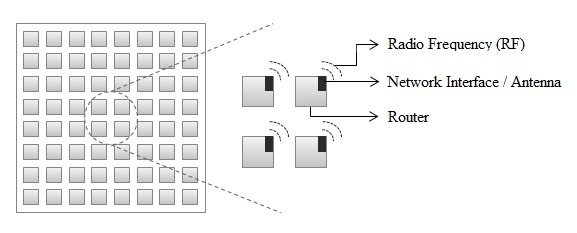
\includegraphics[width=.85\textwidth]{imagem/winoc.jpg}
  % Caption centralizada
  \captionsetup{justification=centering}
  \captionfont{\small{\textbf{\\Fonte: \cite{OliveiraIadis:2011}}}}	
  \label{fig:ComponentesWiNoC}
  \end{figure}


  Os comandos abaixo são usados para apresentação de gráficos. A diferença está apenas na definição do tipo ``grafico`` 
  que permite a adição dos itens no índice de gráficos de forma automática. Os parâmetros são semelhantes aos usados para
  representação de figuras. O parâmetro \textit{width} determina o tamanho do gráfico. O texto entre colchetes 
  no \textit{caption} será o exibido no índice de gráficos e o texto contido entre chaves será exibido na legenda.

\begin{grafico}[H]
  % Alterar espaçamentos antes e depois do caption
  \setlength{\abovecaptionskip}{5pt}
  \setlength{\belowcaptionskip}{0pt}
  % Caption
  \caption[Percentual de pacotes enviados]
	  {Percentual de pacotes enviados}
  \centering
  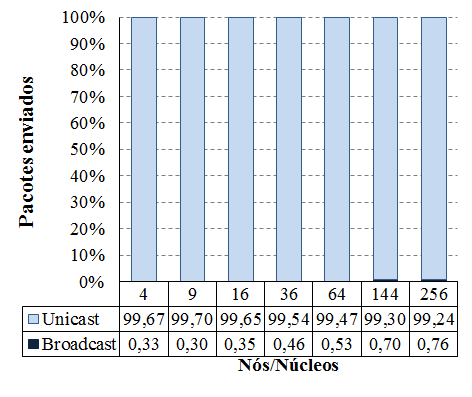
\includegraphics[width=.48\textwidth]{imagem/graficos/grafico_pacotes_enviados_bt.png}
  % Caption centralizada
  \captionsetup[grafico]{justification=centering}
  % Fonte
  \captionfont{\small{\textbf{\\Fonte: Dados da pesquisa}}}
  \end{grafico}

  O Gráfico \ref{graf:quad} mostra os gráficos dispostos lado a lado. Neste caso, componentes \textit{subfloat}
  são utilizados para definir a apresentação em quatro quadrantes. Neste caso, os gráficos podem ser referenciados por conjunto,
  como Gráfico \ref{graf:quad}, ou por um quadrante específico, como Gráfico \ref{graf:injecao_bt}. 

\begin{grafico}[H]
  % Alterar espaçamentos antes e depois do caption
  \setlength{\abovecaptionskip}{5pt}
  \setlength{\belowcaptionskip}{0pt}
  % Caption
  \caption[Resultados da carga de trabalho 1]
	  {Resultados da carga de trabalho 1}
  \centering
  \subfloat[Enviados]
      {\label{graf:enviados_bt}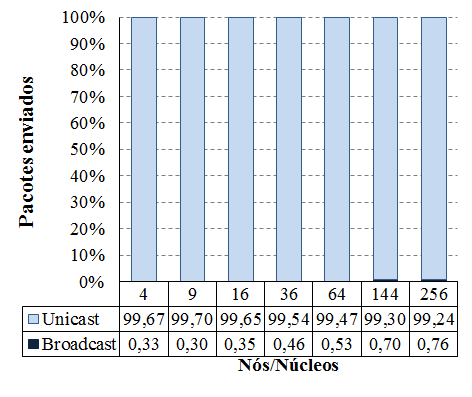
\includegraphics[width=.48\textwidth]{imagem/graficos/grafico_pacotes_enviados_bt.png}} \quad
  \subfloat[Perdidos]
      {\label{graf:perdidos_bt}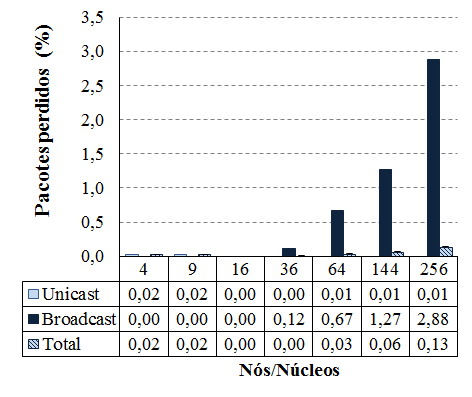
\includegraphics[width=.48\textwidth]{imagem/graficos/grafico_pacotes_perdidos_bt.png}} \quad
  \subfloat[Taxa de injeção]
      {\label{graf:injecao_bt}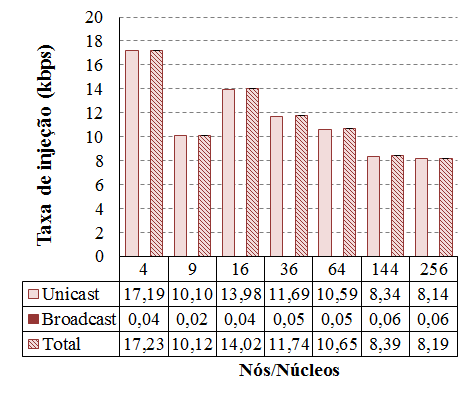
\includegraphics[width=.48\textwidth]{imagem/graficos/grafico_taxa_injecao_bt.png}} \quad
  \subfloat[Vazão]
      {\label{graf:vazao_bt}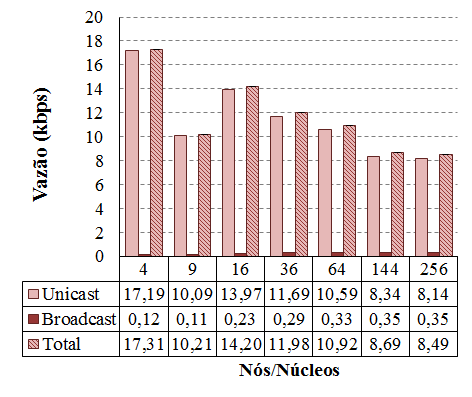
\includegraphics[width=.48\textwidth]{imagem/graficos/grafico_vazao_bt.png}}
  % Caption centralizada
  \captionsetup[grafico]{justification=centering}
  % Fonte
  \captionfont{\small{\textbf{\\Fonte: Dados da pesquisa}}}
  \label{graf:quad}
  \end{grafico}

Um exemplo de criação de tabela é mostrado abaixo. As colunas são separadas por elementos \& e as linhas por duas barras invertidas. 
  Os comandos \textit{hline} e | definem a criação de linhas e colunas para separar os conteúdos, respectivamente. A tabela pode
  ser referenciada usando o comando ref juntamente com o label, como na Tabela \ref{tab:classesNas}. 

   % Tabela
  \begin{table}[H]
    \centering
    \footnotesize
    % Alterar espaçamentos antes e depois do caption
    \setlength{\abovecaptionskip}{0pt}
    \setlength{\belowcaptionskip}{0pt}
    % Caption
    \caption[Parâmetros definidos por classe]{Parâmetros definidos por classe}
    \label{tab:classesNas}
    % Conteúdo da tabela
    \begin{tabular}{c|c|c|c|c|c|c|c}
	\hline \hline
	\textit{Benchmark} &	Parâmetro &	Classe S &	Classe W &	Classe A &	Classe B &	Classe C &	Classe D \\ 
	\hline \hline
 	BT & \textit{Grid}	& $12^3$	& $24^3$ 	& $64^3$	& $102^3$ 	& $162^3$	& $408^3$ \\ 
	CG & Linhas		& 1400		& 7000 		& 14000 	& 75000 	& 150000 	& 1500000 \\ 
	EP & Pares 		& $2^{24}$	& $2^{25}$	& $2^{28}$	& $2^{30}$	& $2^{32}$	& $2^{36}$ \\
	FT & \textit{Grid}	& $64^3$	& $128^2*32$	& $256^2*128$	& $512*256^2$	& $512^3$	& $2048*1024^2$ \\ 
	IS & Chaves		& $2^{16}$	& $2^{20}$	& $2^{23}$	& $2^{25}$	& $2^{27}$	& $2^{31}$ \\ 
	LU & \textit{Grid}	& $12^3$	& $33^3$	& $64^3$	& $102^3$	& $162^3$	& $408^3$ \\
	MG & \textit{Grid}	& $32^3$	& $128^3$	& $256^3$	& $256^3$	& $512^3$	& $1024^3$ \\ 
	SP & \textit{Grid}	& $12^3$	& $36^3$	& $64^3$	& $102^3$	& $162^3$	& $408^3$ \\
	\hline \hline
    \end{tabular}
    % Fonte
    \captionfont{\small{\textbf{\\Fonte: Adaptado de \cite{Nas:2011}}}}
  \end{table}
% Nome do capítulo
\chapter{Observações importantes}
% Label para referenciar
\label{cap3}

% Diminuir espaçamento entre título e texto
\vspace{-1.9cm}

% Texto do capítulo

  Este documento foi compilado em ambiente linux (Ubuntu 10.04) usando o programa Kile - an Integrated LaTeX Environment - Version 2.0.85.
  Para correta formatação os seguintes arquivos do pacote \textit{abntex} devem ser alterados.

    \begin{compactitem}
      \item[a)] Arquivo abnt.cls

      No Ubuntu o arquivo fica armazenado em \textit{/usr/share/texmf/tex/latex/abntex}.
      Comentar a linha 967: Linha comentada para reduzir o espaçamento entre o topo da página e o título.
      Alterar a linha 1143: Parâmetro alterado de 30pt para -30pt para reduzir o espaçamento entre o top da página e o título do apêndice.
      Alterar a linha 985: Parâmetro alterado de 0pt para -30pt para reduzir o espaçamento entre o top da página e o título.
      Alterar a linha 991: Parâmetro alterado de 45pt para 30pt para reduzir o espaçamento entre o texto e o título.

      \item[b)] Arquivo acronym.sty

      No Ubuntu o arquivo fica armazenado em \textit{/usr/share/texmf-texlive/tex/latex/acronym}.
      Alterar a linha 225: Inserir o separador -- entre acrônimo/descrição e remover o negrito com o \textit{normalfont}.
      %\item[\protect\AC@hypertarget{#1}{\acsfont{\normalfont{#2}}} --] #3 

    \end{compactitem}

% PÓS-TEXTUAIS %%
% Bibliografia no arquivo 'Dissertacao.bib'
% Alterar o título das referências para somente 'Referências'
\renewcommand{\bibname}{Referências}
%\bibliographystyle{abnt-alf}
%\bibliography{Dissertacao}

% Para forçar que os apêndices e anexos comecem no anverso
%\setboolean{@openright}{true}

\apendice
\begin{apendice}
%------------------------------------------------------------------------------------------------------------------------------------------------------
% Reiniciar numeração das figuras que aparecem no apêndice
\setcounter{figure}{0}

\chapter{Primeiro apêndice}
\label{apend:express-skel}

% Para diminuir espaçamento entre o título e o texto
\vspace{-1.9cm}

\lstinputlisting[
  language=c, 
  label=leitura-arquivos-diretorio-node, 
  caption={Fonte: \cite{pereira}. O inferno em chamadas de retorno}
]{pos-texto/leitura-arquivos-diretorio-node.js}

\lstinputlisting[
  language=c, 
  label=leitura-arquivos-diretorio-node-callback-heaven, 
  caption={Fonte: \cite{pereira}. Chamadas de retorno organizada}
]{pos-texto/leitura-arquivos-diretorio-node-callback-heaven.js}

\lstinputlisting[
  language=c, 
  label=leitura-arquivos-diretorio-node-strongloop, 
  caption={Fonte: \cite{strongloop}. Exemplo complexo de leitura de arquivos com callbacks hell}
]{pos-texto/leitura-arquivos-diretorio-node-strongloop.js}

\lstinputlisting[
  language=c, 
  label=leitura-arquivos-diretorio-node-strongloop-modular, 
  caption={Fonte: \cite{strongloop}. Exemplo complexo de leitura de arquivos modularizado}
]{pos-texto/leitura-arquivos-diretorio-node-strongloop-modular.js}

\lstinputlisting[
  language=c, 
  label=node-js-app, 
  caption={Fonte: Autor. Arquivo central para aplicação Node}
]{pos-texto/app.js}

\lstinputlisting[
  language=c,
  label=node-js-contact-route, 
  caption={Fonte: Autor. Módulo para a API de contato}
]{pos-texto/contacts.js}
\end{apendice}

\anexo
% Nome do Anexo
\chapter{Primeiro Anexo}
\label{primeiro-anexo}
% Para diminuir espa�amento entre o t�tulo e o texto
\vspace{-1.9cm}

% Texto
% Textos ou documentos não elaborados pelo autor.

\lstinputlisting[
  language=c, 
  label=leitura-arquivos-diretorio-node, 
  caption={Fonte: \cite{Pereira:2013}. O inferno em chamadas de retorno}
]{pos-texto/leitura-arquivos-diretorio-node.js}

\lstinputlisting[
  language=c, 
  label=leitura-arquivos-diretorio-node-callback-heaven, 
  caption={Fonte: \cite{Pereira:2013}. Chamadas de retorno organizada}
]{pos-texto/leitura-arquivos-diretorio-node-callback-heaven.js}

\lstinputlisting[
  language=c, 
  label=leitura-arquivos-diretorio-node-strongloop, 
  caption={Fonte: \cite{Strongloop:2013}. Exemplo complexo de leitura de arquivos com callbacks hell}
]{pos-texto/leitura-arquivos-diretorio-node-strongloop.js}

\lstinputlisting[
  language=c, 
  label=leitura-arquivos-diretorio-node-strongloop-modular, 
  caption={Fonte: \cite{Strongloop:2013}. Exemplo complexo de leitura de arquivos modularizado}
]{pos-texto/leitura-arquivos-diretorio-node-strongloop-modular.js}


\end{document}